\documentclass[12pt]{article}

% Packages
% ---
\usepackage{amsmath} % Advanced math typesetting
\usepackage[utf8]{inputenc} % Unicode support (Umlauts etc.)
\usepackage[french]{babel} % Change hyphenation rules
\usepackage{hyperref} % Add a link to your document
\usepackage{graphicx} % Add pictures to your document
\usepackage{listings} % Source code formatting and highlighting
\usepackage{fancybox}
\usepackage{subfig}
\usepackage[margin=1in]{geometry}
\usepackage{wrapfig}

%\DeclareGraphicsExtensions{.png}
\captionsetup[figure]{textfont=it}

\title{Rapport du travail pratique 3 : Interpolation et extrapolation}
\date{\today}
\author{Présenté par Philippe Caron\\dans le cadre du cours Traitement du signal (IFT3205)\\Université de Montréal}

\begin{document}
\begin{titlepage}
  \maketitle
  \thispagestyle{empty}
\end{titlepage}

\setcounter{section}{1}
\section{Interpolation spectrale}
%\setcounter{subsection}{1}
\subsection{Calcul des images agrandies}
Voici les images obtenues en utilisant respectivement l'interpolation au plus proche voisin (a), l'interpolation bi-linéaire (b), puis l'interpolation spectrale (c).

\begin{figure}[ht]
  \centering
  \subfloat[]{\shadowbox{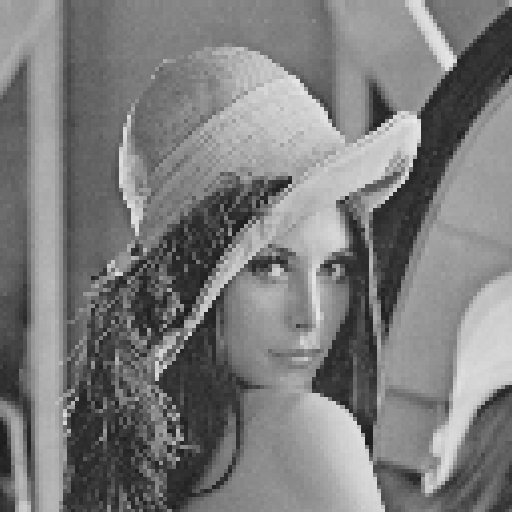
\includegraphics[height = 4.7cm]{image-TpIFT3205-2-1a.png}}}
  \hspace{0.1cm}
  \subfloat[]{\shadowbox{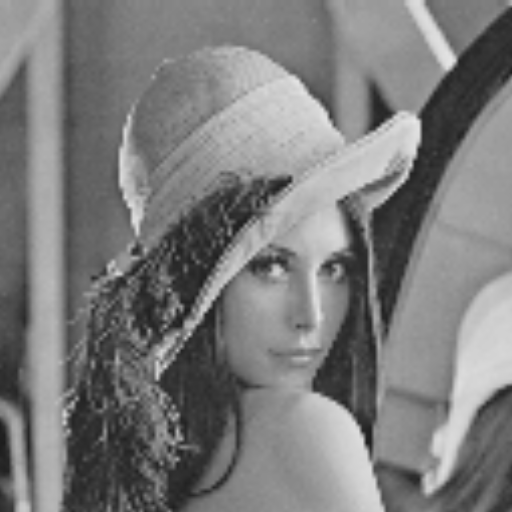
\includegraphics[height = 4.7cm]{image-TpIFT3205-2-1b.png}}}
  \hspace{0.1cm}
  \subfloat[]{\shadowbox{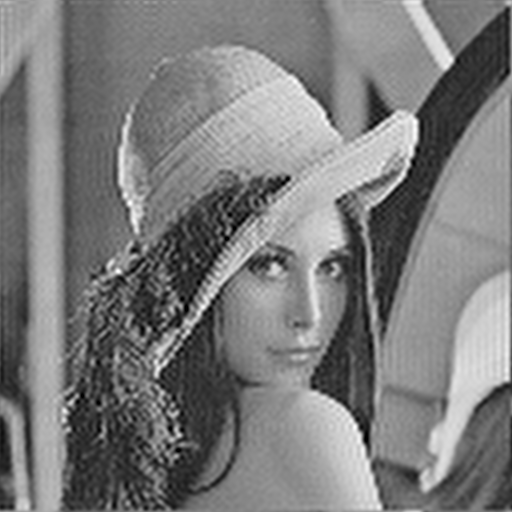
\includegraphics[height = 4.7cm]{image-TpIFT3205-2-1c.png}}}
  \captionsetup{width=.8\linewidth}
  \caption{L'image lena128.pgm agrandie de trois manière différentes}
\end{figure}

À première vue, l'interpolation bi-linéaire semble la plus appropriée étant donné qu'elle semble mieux conserver l'aspect de l'image que les deux autres. Mais si on s'y attarde plus longtemps, on remarque un effet de «flou» sur celle-ci qui ne se trouve pas sur l'image obtenue par interpolation spectrale. En effet, on remarque que sur celle-ci les blancs sont plus blancs et les noirs plus noirs, et on n'a pas perdu la texture (voir plumes ou chapeau). Il n'est donc pas difficle de croire que l'interpolation spectrale soit optimale.

\subsection{Facteur de normalisation}
Ce qu'on fait en calculant l'interpolation spectrale est simplement de placer le spectre dans un gabari de la taille de la nouvelle image. Or cette méthode ne respecte pas la conservation de l'énergie. En effet, il suffit de visualier le processus pour comprendre; on colle une image de 128x128px dans une image de 512x512px, il y a donc 16 fois plus de pixels sur l'image de destination que sur l'image source. Puisque l'énergie contenue dans les 128x128 pixels devra alimenter tout la grille de 512x512, en multipliant ceux-ci par 16, on obtiendra une image de la même luminosité qu'avant. De manière plus générale, on peut calculer ce facteur en faisant le rapport des aires:

\begin{equation}
  F_n = \frac{l_s \cdot h_s}{l_d \cdot h_d}
\end{equation}
Où $l_s$ et $h_s$ sont la largeur et la hauteur source et $l_d$ et $h_d$ sont la largeur et la hauteur de destination.

\subsection{Augmentation du spectre}
Le plus simple serait de placer le spectre 128x128 dans une image vide 512x512, calculer la transformée de Fourrier sur le spectre, multiplier l'image obtenue par le facteur de normalisation, et faire la transformée de Fourrier inverse. Cependant, cela revient à calculer l'image finale. S'il ne faut pas calculer l'image agrandie, cela signifie qu'on ne peut pas utiliser la transformée de Fourrier inverse sur le spectre, cette approche est donc impossible.

On pourrait tenter d'extrapoler le spectre, mais cela ne fonctionnerait probablement qu'avec le module. Puisqu'il est complexe, la partie réelle et la partie imaginaire sont individuellement plutôt aléatoires, ce qui rend l'extrapolation très difficle (voire impossible). Sans compter que cette méthode ajouterait de la fausse information à l'image, qui peut-être la rendrait plus agréable à l'oeil, mais dans certains contextes pourrait la rendre moins intéressante.

On peut cependant appliquer directement le facteur de normalisation au spectre avant d'effectuer la transformée de fourrier sur celui-ci. Le processus complet serait donc: center le spectre de 128x128, le placer au centre d'une image vide (tout les pixels à 0), recentrer la nouvelle image de 512x512, multiplier chacun des pixels par 16. De cette manière on aurait un spectre équivalent à 4 fois le spectre précédent, sans aucune fausse information ajoutée.

\pagebreak

\section{Interpolation spectrale par seuillage}
Voici les images calculées à chaque itération:
\begin{figure}[ht]
  \centering
  \subfloat[]{\shadowbox{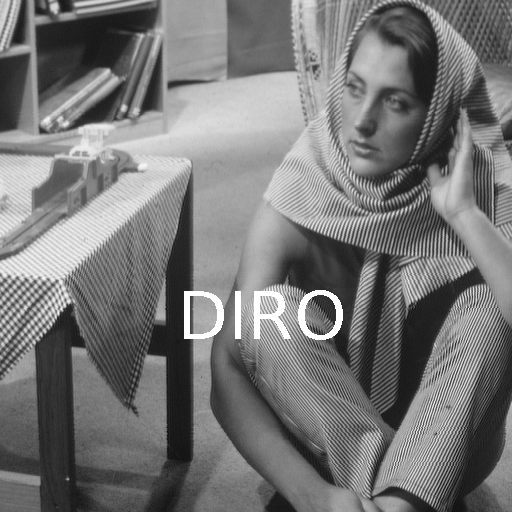
\includegraphics[height = 4.7cm]{image-TpIFT3205-3-2-0.png}}}
  \hspace{0.1cm}
  \subfloat[]{\shadowbox{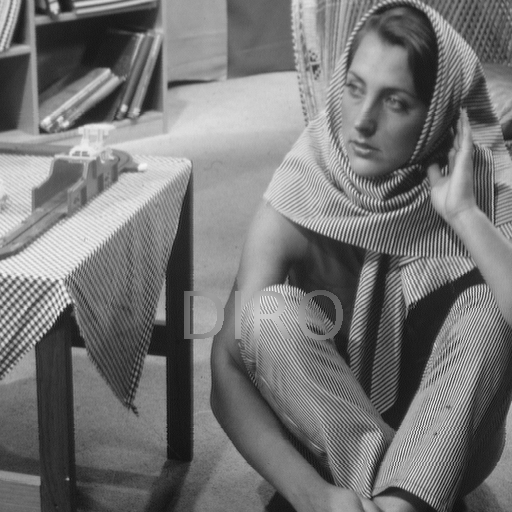
\includegraphics[height = 4.7cm]{image-TpIFT3205-3-2-1.png}}}
  \hspace{0.1cm}
  \subfloat[]{\shadowbox{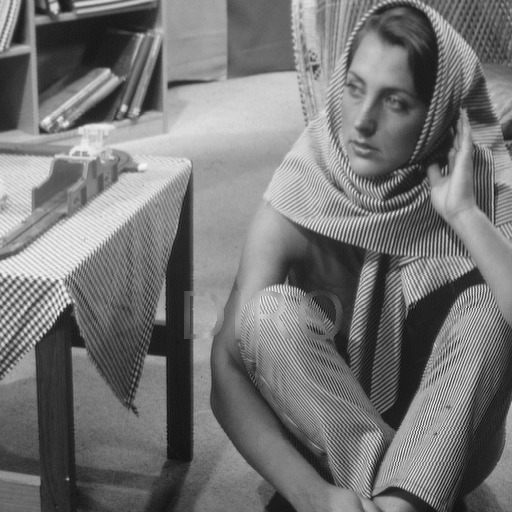
\includegraphics[height = 4.7cm]{image-TpIFT3205-3-2-2.png}}}
  \hspace{0.1cm}
  \subfloat[]{\shadowbox{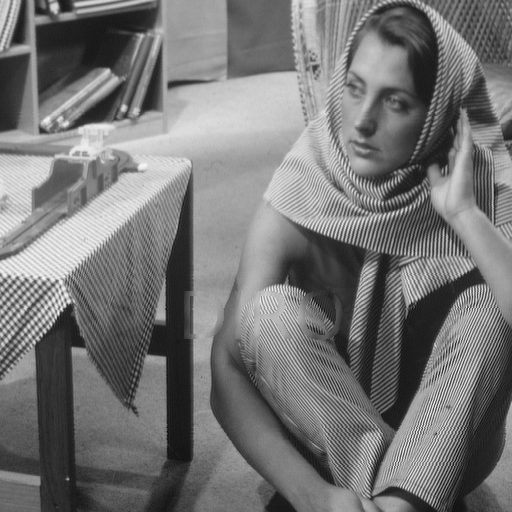
\includegraphics[height = 4.7cm]{image-TpIFT3205-3-2-3.png}}}
  \hspace{0.1cm}
  \subfloat[]{\shadowbox{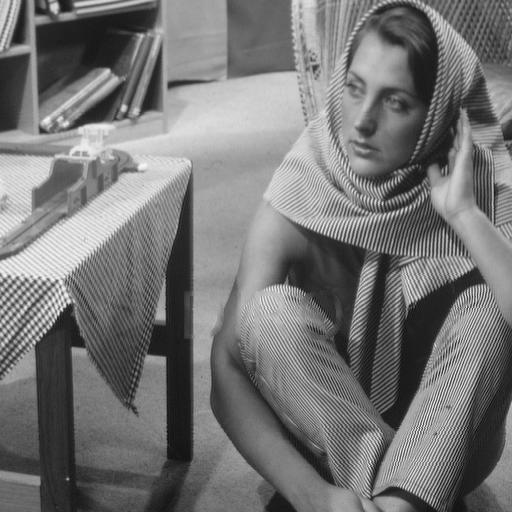
\includegraphics[height = 4.7cm]{image-TpIFT3205-3-2-4.png}}}
  \hspace{0.1cm}
  \subfloat[]{\shadowbox{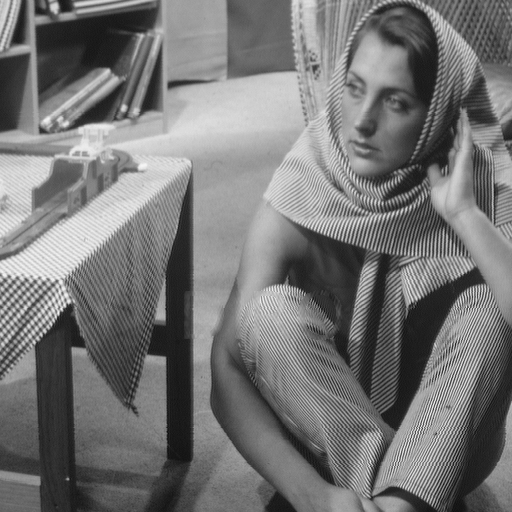
\includegraphics[height = 4.7cm]{image-TpIFT3205-3-2-5.png}}}
  \captionsetup{width=.8\linewidth}
  \caption{Les itérations 0 à 5 du processus d'interpolation}
\end{figure}

\setcounter{subsection}{1}
\subsection{Calcul des images}
Pour calculer les images, un programme qui détermine automatiquement la position des images à chaque itération a été utilisé. L'objectif étant éventuellement de pouvoir l'utiliser en faisant bien plus que 5 itérations, et d'améliorer la qualité du rendu. Pour se faire, il place la dégradation dans le coin de chacune des «sous-images» s'assurant que ce soit un coin différent à chaque fois. Il prend également en paramètre la valeur de seuil en pourcentage, qu'il divise par deux à chaque itération.

\pagebreak
\subsection{Fonctionnement de la méthode}
Les lettres «DIRO» en blanc pur sont évidemment très différentes du reste de l'image, il n'est donc pas surprenant que les fréquences qui contribuent à les afficher soient très faible. Le but de cette méthode est justement d'isoler les fréquences plus faibles afin de retrouver le détail sous-jacent. À chaque itération, les fréquences les plus faibles sont éliminées, ce qui produit une image un peu floue, sans détail, mais dont l'aspect général est uniforme. En remplaçant l'intérieur des lettres par cette image, on les rend plus cohérentes avec le reste de l'image. Pour conséquence, les lettres sont de moins en moins visibles, et les fréquences qui les composent sont donc de moins en moins importantes. Ceci permet de diminuer la valeur du seuil. Plus le seuil diminue, plus l'image produite est détaillée; les fréquences environnantes vont alors contribuer de plus en plus à ce qui se trouve à l'intérieur des lettres. C'est pourquoi éventuellement, on aura l'impression que les lettres ont disparues; leurs fréquences originales auront toutes été suprimées, tandis qu'elles seront remplacées par les fréquences de leur entourage (qui on suppose sont représentatives de l'intérieur). Et effectivement, hormis quelques accrocs, le résultat fini semble très près de la réalité.

\pagebreak

\section{Extrapolation spectrale par seuillage}
\subsection{Stratégie d'extrapolation}
Pour extrapoler le haut des images, la même méthode qu'au numéro 3 sera utilisée, c'est-à-dire le seuillage. Ici, nous considérerons simplement que les 50 lignes du haut à extrapoler sont le défaut. Toutefois pour augmenter les chances de succès, plusieurs prétraitement et paramètres seront choisis à l'avances:

\subsubsection{Technique de remplissage}
Afin d'éviter les lignes verticales sur les images produites (celles qui ressemblent à des lignes d'imprimantes sur les photos de la donnée du TP), au lieu de remplacer chaque colonnes par la moyenne des 30 dernières lignes, chaque lignes ajoutée est en fait la précédente à laquelle un filtre spatial [ 1 2 1 ] a été appliqué. En voici le résultat:

\begin{figure}[ht]
  \centering
  \shadowbox{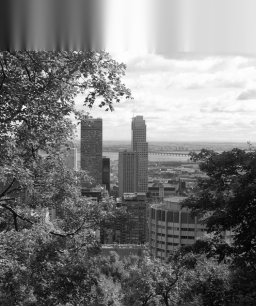
\includegraphics[width = 5cm]{image-TpIFT3205-4-1-prel.png}}
  \captionsetup{width=.8\linewidth}
  \caption{Image remplie grace à la technique du filtre spatial}
\end{figure}

\subsubsection{Choix de l'échantillon}
Puisqu'il ne faut qu'extrapoler les 50 dernières lignes, et que dans la plupart des cas l'information contenue dans le bas des images est sans valeur, le programme d'extrapolation ne considérera que les 120 lignes précédentes (choix arbitraire). L'important était simplement que l'échantillon soit un peu plus gros que 2 fois l'extrapolation.

\subsubsection{Nombre d'itération}
Après quelques test, 7 a été choisi comme nombre d'itération. C'est l'itération à partir de laquelle les itérations successive semblaient avoir très peu d'effet, mais qui elle-même avait encore un effet significatif, tout en étant exécutable en un temps raisonnable ($\approx$10-15s).

\pagebreak
\subsection{Résultats}
Voici les résultats obtenus en utilisant pour chaque image le même programme (démontrant sont efficacité plus ou moins universelle):
\begin{figure}[ht]
  \centering
  \subfloat[Image originale]{\shadowbox{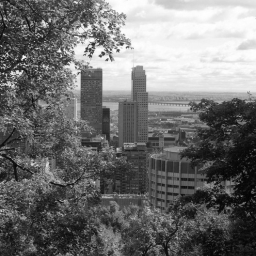
\includegraphics[width = 5cm]{ParcMontRoyal.png}}}
  \hspace{1cm}
  \subfloat[Image extrapolée]{\shadowbox{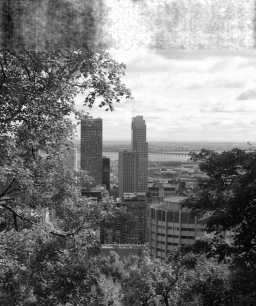
\includegraphics[width = 5cm]{image-TpIFT3205-4-1.png}}}
  \captionsetup{width=.8\linewidth}
  \caption{Parc du Mont-Royal}
\end{figure}
\begin{figure}[ht]
  \centering
  \subfloat[Image originale]{\shadowbox{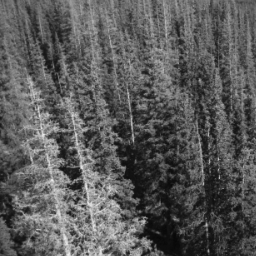
\includegraphics[width = 5cm]{Img1.png}}}
  \hspace{1cm}
  \subfloat[Image extrapolée]{\shadowbox{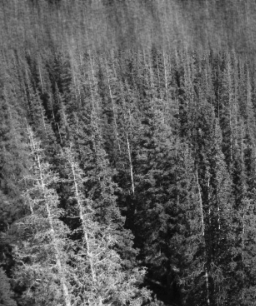
\includegraphics[width = 5cm]{image-TpIFT3205-4-1a.png}}}
  \captionsetup{width=.8\linewidth}
  \caption{Forêt de sapins}
\end{figure}
\begin{figure}[ht]
  \centering
  \subfloat[Image originale]{\shadowbox{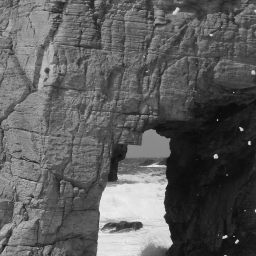
\includegraphics[width = 5cm]{Img2.png}}}
  \hspace{1cm}
  \subfloat[Image extrapolée]{\shadowbox{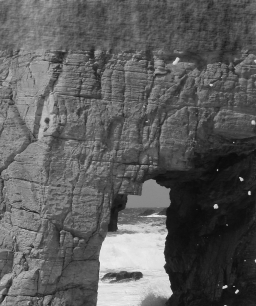
\includegraphics[width = 5cm]{image-TpIFT3205-4-1b.png}}}
  \captionsetup{width=.8\linewidth}
  \caption{Roché percé}
\end{figure}
\begin{figure}[ht]
  \centering
  \subfloat[Image originale]{\shadowbox{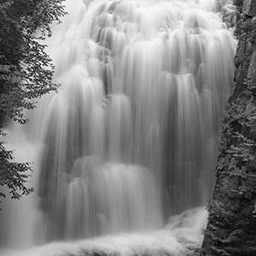
\includegraphics[width = 5cm]{Img3.png}}}
  \hspace{1cm}
  \subfloat[Image extrapolée]{\shadowbox{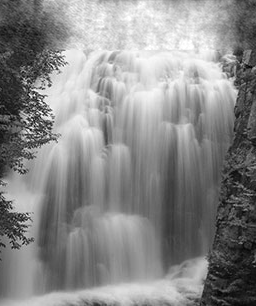
\includegraphics[width = 5cm]{image-TpIFT3205-4-1c.png}}}
  \captionsetup{width=.8\linewidth}
  \caption{Chutes}
\end{figure}
\begin{figure}[ht]
  \centering
  \subfloat[Image originale]{\shadowbox{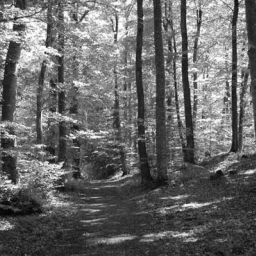
\includegraphics[width = 5cm]{Img4.png}}}
  \hspace{1cm}
  \subfloat[Image extrapolée]{\shadowbox{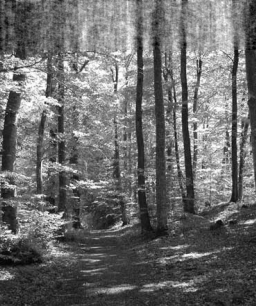
\includegraphics[width = 5cm]{image-TpIFT3205-4-1d.png}}}
  \captionsetup{width=.8\linewidth}
  \caption{Clairière}
\end{figure}
\end{document}

